\documentclass{article}

\usepackage{fancyhdr}
\usepackage{extramarks}
\usepackage{amsmath}
\usepackage{amsthm}
\usepackage{amsfonts}
\usepackage{tikz}
\usepackage{graphicx}
\usepackage{float}
\usepackage{listings}
\usepackage{booktabs}
\usepackage{hyperref}

%\usetikzlibrary{automata,positioning}
\usetikzlibrary{shapes, arrows}

%
% Basic Document Settings
%

\definecolor{navyblue}{rgb}{0.0, 0.0, 0.5}
\definecolor{oxfordblue}{rgb}{0.0, 0.15, 0.40}
\hypersetup{colorlinks, breaklinks, urlcolor=oxfordblue, linkcolor=oxfordblue, citecolor=oxfordblue}

\topmargin=-0.45in
\evensidemargin=0in
\oddsidemargin=0in
\textwidth=6.5in
\textheight=9.0in
\headsep=0.25in

\linespread{1.1}

\pagestyle{fancy}
\lhead{\hmwkAuthorName}
\rhead{\hmwkClass\ (\hmwkClassInstructor)}
\cfoot{\thepage}

\lstset{
  caption=\lstname,
  %backgroundcolor=\color{lightgray},
  literate={\$}{{\$}}1,
  breaklines=true,
  basicstyle=\ttfamily\small
}

\DeclareMathOperator*{\argmin}{arg\,min}
\DeclareMathOperator*{\argmax}{arg\,max}
\renewcommand\headrulewidth{0.4pt}
\renewcommand\footrulewidth{0.4pt}

\setlength\parindent{0pt}

\newcommand{\hmwkTitle}{Utilizing reinforcement learning techniques to play Atari's Breakout}
\newcommand{\hmwkDueDate}{07 December 2015}
\newcommand{\hmwkClass}{Reinforcement Learning}
\newcommand{\hmwkClassInstructor}{Dr. Itamar Arel}
\newcommand{\hmwkAuthorName}{Andrew Messing, Ben Brock, and Cory Walker}

%
% Title Page
%

\title{
    \vspace{2in}
    \textmd{\textbf{\hmwkTitle}}\\
    \normalsize\vspace{0.1in}\small{Due\ on\ \hmwkDueDate}\\
    \vspace{0.1in}\large{\textit{\hmwkClassInstructor}}
    \vspace{3in}
}

\author{\textbf{\hmwkAuthorName}}
\date{}

\renewcommand{\part}[1]{\textbf{\large Part \Alph{partCounter}}\stepcounter{partCounter}\\}

%
% Various Helper Commands
%

% Alias for the Solution section header
\newcommand{\solution}{ \hfill \break \break \textbf{Solution} \hfill \break \break}

\begin{document}

\maketitle

\pagebreak

\begin{abstract}
We demonstrate the performance of two different reinforcement learning methods, basic Q-learning using manual image processing and deep Q-learning using raw pixel input, on Atari's Breakout.  While deep reinforcement learning techniques may be generalizable across games and ultimately result in optimal performance, they require a large amount of computational resources and time for training.  By performing manual image processing to derive states, we show that similar performance can be achieved in less time using basic Q-learning.
\end{abstract}

\section{Introduction}
Deep Reinforment Learning is a relatively new approach to learn to control agents via high dimensional sensory inputs like vision and speech. This project compares the success of a specific feature based reinforcement learning approach to a deep reinforcement learning one using the atari game Breakout and the Arcade Learning Environment.

\section{Breakout and feature extraction}
\subsection{Breakout}
Breakout is a classic arcade game developed by Atari, Inc. Similar to pong the objective is to use a paddle to bounce a ball; however for breakout the paddle moves horizontally and is positioned at the bottom of the screen. At the top of the screen are multiple layers of bricks. Everytime the ball collides with a brick it breaks it and the player gains points. The goal of the game is to break all the bricks, score points, and not let the ball fall below the paddle as that costs the user a life. When all the lives are gone the game is over.

\begin{figure}[H]
  \centering
  \caption{The Breakout setup.}
  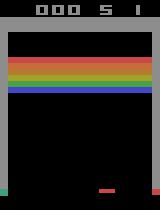
\includegraphics[width=50mm]{tmp.jpg}
  \label{breakout:simple}
\end{figure}

\subsection{Arcade Learning Environment}
The Arcade Learning Environment (ALE) is a simple object-oriented framework designed to allow researchers to test Artificial Intelligence agents to play Atari 2600 games \cite{ale}. The agent can receive the game frames and ram and is given access to the number of lives, the score, and other information from the game. Then the agent can use this to come with an action that it would send back to the ALE. The controller that is simulated contains a joystick, an action button, and a couple of menu buttons that total to about 20 possible actions including the buttons being pressed and the joystick being moved in one of eight directions.
\\\\
For breakout specifically there are three actions that contribute to the game: move the joystick left, move the joystick right, and do nothing.

\subsection{Feature Extraction}
To extract features for the basic reinforcement learning agent, we used image processing to capture the position of the paddle and ball.  See Figure \ref{breakout:fe} for a visualization of the results of the feature extraction.  While the paddle maintained one of two colors making it relatively easy to extract, the ball changes colors as it goes by each of the brick layers, taking on the color of each brick layer.  When the ball is in open space, it returns to the color of the paddle. 

\begin{figure}
  \centering
  \caption{Feature extraction performed on a frame from Breakout.  The white dots indicate the detected x and y coordinates of the paddle and ball.}
  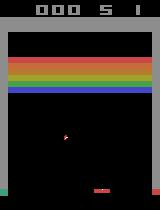
\includegraphics[width=50mm]{tmp2.jpg}
  \label{breakout:fe}
\end{figure}

\section{Reinforcement learning}
\subsection{Introduction}
The Breakout problem is the problem of playing the game of Breakout while maximizing the score received.  Our RL agent controls the paddle and, at each timestep of the ALE engine, has three possible actions: to move the paddle to the left, to hold the paddle still, or to move the paddle to the left.  The optimal action will depend depend on the position of the paddle, the position of the ball, and possibly the position of the blocks overhead.  Here, we will present a simple Q-learning approach to solving the Breakout problem.  First, we will discuss the formulation of the problem as a Markov Decision Process (MDP), then the design and implementation of our Q-learning approach to training an RL agent to solve Breakout.  Then, we will discuss the training results and performance of our agent.
\subsection{Formulation as an MDP}
In our formulation of Breakout, the RL agent has three possible states, which are each derived from the relative x-coordinate position of the ball and paddle.  Either the ball is to the left of the paddle (state 1), the ball is directly on top of the paddle (state 2), or the ball is to the right of the paddle (state 3).  In our formulation, our RL agent is given a state value and the opportunity to perform an action at each timestep of the ALE.  The RL agent may perform one of three actions: the RL agent may choose to move the paddle to the left, to the right, or to hold the paddle still.  When the ball drops below the paddle (losing a game life), the RL agent will receive a reward of -10.  At all other timesteps, the RL agent will receive a reward of 0.  An episode begins when a game of Breakout starts and ends when the game has ended (the agent loses all of its lives).
\\\\
We have chosen this formulation because of its simplicity.  While a truly optimal Breakout player may use the position of the bricks to inform its decisions about how to hit the ball, it is our hypothesis that a player which simply attempts to hit the ball may be very nearly optimal.  We wish to demonstrate that a very simple formulation may achieve high performance if it is well-tuned to the attributes of the system.
\subsection{Q-Learning Method}
We use Q-learning with elligibility traces to train our RL agent to solve Breakout \cite{sutton}.  For data structures, we keep a vector $Q(s, a)$ of state-action values.  For each episode, we also maintain a vector $e(s, a)$ of elligibility traces for each state-action pair.  When we initialize our RL agent, we initialize our $Q$ vector with random values between 0 and 1.  At the start of each episode, we initialize an elligibility trace $e(s, a)$ with all zeros.  Then, for each step, we discover the current state $s$ using our custom image processing.  The agent remembers a previous action $a$ from the last timestep.  Then, the agent picks a new action $a'$ from $Q(s, a)$ using an $\epsilon$-greedy policy.  From this action, the agent observes a reward $r$.  The agent estimates a change in state value, $\delta$, using the reward $r$ and the difference in state values.  It then increases the elligibility of the current state $s$.  Then, for every state, the agent will update the value of the state in accordance with its elligibility and the difference in state value $\delta$ the agent just experienced.  See Figure \ref{qlearn:code} for a concise technical description of the RL method used.

\begin{figure}
    \centering
    \caption{Q-learning method used to train our RL agent.}
    \begin{itemize}
    \item[] Initialize $Q(s, a)$ arbitrarily
    \item[] For each episode:
    \item[] \hspace{2em} $e(s, a) \leftarrow 0$
    \item[] \hspace{2em} For each step:
    \item[] \hspace{4em} Discover current state $s$ with IP, choose action $a$
    \item[] \hspace{4em} Choose $a'$ from $Q(s, a)$ ($\epsilon$-greedy)
    \item[] \hspace{4em} Take action $a'$, observe $r$ and $s'$
    \item[] \hspace{4em} $\delta \leftarrow r + \gamma Q(s', a') - Q(s, a)$
    \item[] \hspace{4em} $e(s, a) \leftarrow e(s, a) + 1$
    \item[] \hspace{4em} For all $s, a$:
    \item[] \hspace{6em} $Q(s, a) \leftarrow Q(s, a) + \alpha \delta e(s, a)$
    \item[] \hspace{6em} $e(s) \leftarrow \gamma \lambda e(s)$
    \item[] \hspace{4em} $s \leftarrow s'$
  \end{itemize}
  \label{qlearn:code}
\end{figure}

\subsection{Results}
\subsubsection{Hyperparameters}
We trained our RL agent using the hyperparameters $\alpha = 0.01$, $\gamma = 0.9$, $\lambda = 0.9$, and $\epsilon = 0.01$.  We started off with hyperparameters of $\alpha = 0.1$, $\gamma = 0.7$, $\lambda = 0.9$, and $\epsilon = 0.1$ and randomly modified them until we arrived at the new hyperparameters, which train and converge much more readily than the original ones.  A major problem with the original hyperparameters was that the agent would converge very quickly to what we could observe is a good policy, then diverge from it, randomly cycling through subpar policies.  Lowering the step size $\alpha$ resulted in more stable training.  We hypothesize that the larger step size is in an issue because of the very large number of times the RL agent visits each state.  We also increased $\gamma$ and $\lambda$, which together control the decay of the elligibility trace.  Because the agent may perform a sub-optimal action and then visit many other states before a negative reward is received (the agent looses a life), it is important that states remain elligible so that a bad state-action pair can be recognized.  In addition, we hypothesize that lowering the value of $\epsilon$ allows bad state-action pairs to be isolated and recognized.
\subsubsection{Training and Performance}
We found that our RL agent, trained with the above hyperparameters, converged to a near-optimal policy after about 50 episodes, which corresponds to about 25 minutes of gameplay.

\section{Deep reinforcement learning}
  While manual feature extraction can result in faster training and potentially better performance, there is a large motivation to be able to learn from general and high dimensional inputs such as video and sound. If we could learn to play Atari games from raw pixels, we could use the same algorithm on an array of games, even games we have never actually played before. \\

  Of course, things are not as simple as creating a state for every possible screen. Since the Atari environment has 128 colors and a 210x160 screen, the number of states resulting from this would be $128^{210 \cdot 160} \approx 1.799\times 10^{70802}$. Even if we reduced the number of colors to 4, we would still have a number with 20,000 digits for the number of states. Furthermore, even if we cut the screen size by a quarter, we would still have $4^{105 \cdot 80} \approx 2.013\times 10^{5057}$ states. \\

  On top of all this, just a single screen in Breakout and many other Atari games is just a partial representation of the game state. The ball could be moving either right or left, which is an important piece of information for scoring points. \\

  Recently Google DeepMind has made progress in this problem space by utilizing convolutional neural networks for estimating the action-value function based on visual input \cite{dmnips}. The rest of this project will describe implementing DeepMind's Double DQN algorithm, an algorithm for which no open-source implementation previously existed.
\subsection{Deep Q network}
  At its core, the Deep Q network is a function approximator for the action-value function. The standard Deep Q network for playing Atari games features around 1.5 million parameters. Each parameter is updated through the following equation:
  \[ \boldsymbol{\theta}_{t+1} = \boldsymbol{\theta}_t+\alpha(Y_t^Q-Q(S_t,A_t;\boldsymbol{\theta}_t))\nabla_{\boldsymbol{\theta}_t}Q(S_t,A_t;\boldsymbol{\theta}_t) \]
  The network is composed of the following stacked sequence of layers:
  \begin{enumerate}
    \item An input layer for the past 4 scaled (84x84) and grayscale snapshots of the screen.
    \item A 2D convolution layer with 32 filters of size 8 and stride 4. The layer uses a ReLU nonlinearity.
    \item A 2D convolution layer with 64 filters of size 4 and stride 2. The layer uses a ReLU nonlinearity.
    \item A 2D convolution layer with 64 filters of size 3 and stride 1. The layer uses a ReLU nonlinearity.
    \item Next we have a fully-connected layer with 512 units. This layer uses a ReLU nonlinearity.
    \item Finally we have another fully-connected layer as the output layer with $|A|$ outputs. This layer uses linear activation.
  \end{enumerate}

\subsection{DQN variations}
DeepMind first presented their version of the Deep Q network at the NIPS Deep Learning Workshop in late 2013 \cite{dmnips}. In this paper they train the network on seven Atari games, surpassing a human expert on three of them. The network described in this paper requires roughly 24 hours of training for a game on a standard GPU.\\

In early 2015, DeepMind published a paper in Nature which updates the network structure originally defined \cite{dmnature}. The new network is similar to the NIPS one, but it features much more conservative hyperparameters (increasing training time to a week) and first describes model freezing. \\

Model freezing is a technique that separates the action-value function into two functions with the same structure but different weights. The main action-value function has weights $\boldsymbol{\theta}_t$ and the target action-value function has weights $\boldsymbol{\theta}_t^-$. Every 10,000 training updates we set $\boldsymbol{\theta}_t^- \leftarrow \boldsymbol{\theta}_t$ to keep the target action-value function in sync with the main one. It is possible that the NIPS version used model freezing as well, but the paper made no mention of it and therefore the implementations of the NIPS-described DQN do not feature model freezing. \\

In September 2015, DeepMind updated the algorithm described in Nature to address value overestimates \cite{dmdoubl}. They call this algorithm Double DQN, and this is the algorithm that we will implement and apply to Atari Breakout.

\subsection{Double DQN formulation}
  The motivation behind Double Q-learning is that max operator uses the same values for action selection and evaluation, which can cause an issue with overoptimistic value estimates, especially with function approximation. If all action-values are uniformly overestimated, this would not affect the policy. The authors of the Double DQN paper argue that the overestimations are not uniform, leading to suboptimal policies. Double Q learning attempts to address these overestimations by decoupling action selection from action evaluation. While traditional Double Q-learning involves training two different value functions, van Hasselt et. al. argue that the same effect can be achieved for DQN with the following change to the target function $Y_t$:

  \[Y_t^{\textrm{DQN}} \equiv R_{t+1} + \gamma \textcolor{red}{\max_{a} Q(S_{t+1},a;\boldsymbol{\theta}_t^-)} \]
  \[ \Downarrow \]
  \[\boxed{Y_t^{\textrm{DoubleDQN}} \equiv R_{t+1} + \gamma \textcolor{red}{Q(S_{t+1},\argmax_a Q(S_{t+1},a;\boldsymbol{\theta}_t),\boldsymbol{\theta}_t^-)}} \]

  We can reason that if $\boldsymbol{\theta}_t^- = \boldsymbol{\theta}_t$, there is no difference between the two equations. This is why Double DQN requires model freezing to work correctly. Since we use the target function $Y_t$ to calcuate the approximation errors with which to train our network, changing this function changes the policies that our network learns. According to the Double DQN authors, these different policies led to higher scores in many games.

\subsection{Implementation}
  We chose to implement Double DQN both because we are interested in the algorithm and also because there were not previously any open source implementations of Double DQN. Only the paper existed. We built on a very good existing open source implementation for vanilla DQN built by Nathan Sprague, \href{https://github.com/spragunr/deep_q_rl}{deep\_q\_rl}. This implementation uses a Lasagne/Theano backend with useful code for model import/export and visualization of the gameplay. It also features an efficient implementation of the replay buffer that uses a circular buffer to store the 1M replay frames. Furthermore, Sprague's implementation already supported the NIPS and Nature algorithms, giving us a baseline with which to compare our results from Double DQN. \\

We performed our testing on an EC2 g2.2xlarge instance equipped with a single NVIDIA Kepler GK104 GPU and 15GB of onboard memory. Our single-threaded program was CPU bound and only used 30\% of the GPU, so it was possible to train another network simultaneously, as long as we reduced the replay buffer size from 8GB to 7GB. One main issue with testing these networks is that they can take up to 12 hours to determine if there is an issue with learning. After a few iterations of making changes and testing them, we arrived with a solution that stayed true to the Double DQN paper and seemed to learn at a good rate. \\

Our open source implementation of Double DQN can be viewed and commented on by visiting the pull request at \href{https://github.com/spragunr/deep_q_rl/pull/52}{https://github.com/spragunr/deep\_q\_rl/pull/52}. The fork with the implementation is located at \href{https://github.com/corywalker/deep_q_rl}{https://github.com/corywalker/deep\_q\_rl}.

\subsection{Results}
We trained both a DQN and a Double DQN on Atari Breakout for about 20 hours:
  \begin{figure}[H]
    \centering
    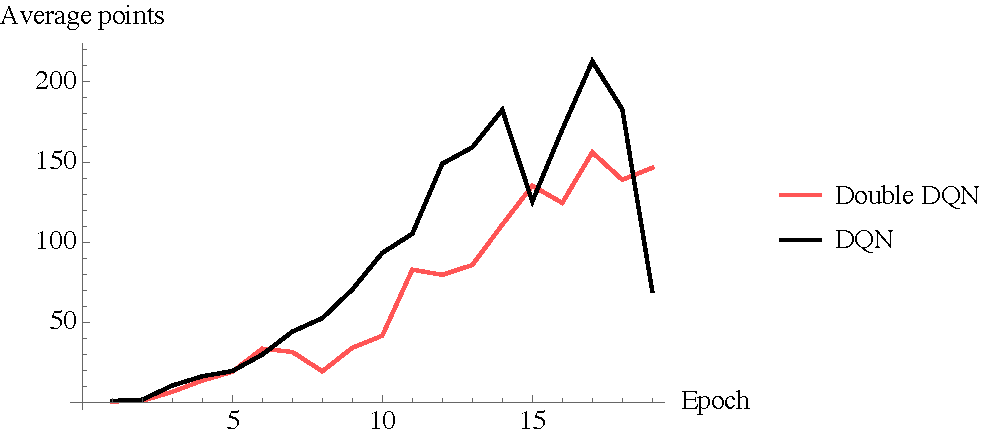
\includegraphics[width=120mm]{dqn_rewardper.pdf}
  \end{figure}
  Each epoch takes about an hour, and we only trained for a few epochs out of the recommended 200. The performance comparison between DQN and Double DQN for Breakout is inconclusive for Breakout after just 20 epochs. This should be expected since the Double DQN paper reported roughly equivalent performance for Breakout. Ideally, we should have picked a game with more pronounced difference for Double DQN, such as Space Invaders. The number of training steps per epoch is 250000, and we skip every 4 frames, meaning that each epoch is actually 1M frames. Since the ALE is 60fps, each epoch is equivalent to ~278 minutes of gameplay. The DeepMind paper quoted Breakout human performance at 30 points per episode. Since it seems to take 6 epochs to reach this (in both Double DQN and DQN), we estimate that this is $6 \cdot 278 = 1668 \mbox{ mins} = 27.8 \mbox{ hours}$ of gameplay to reach human level performance. In terms of computation time, it takes about an hour or two. \\

  The plots of the mean value estimates indicate that Double DQN accomplishes its purpose of mitigating value overestimation:
  \begin{figure}[H]
    \centering
    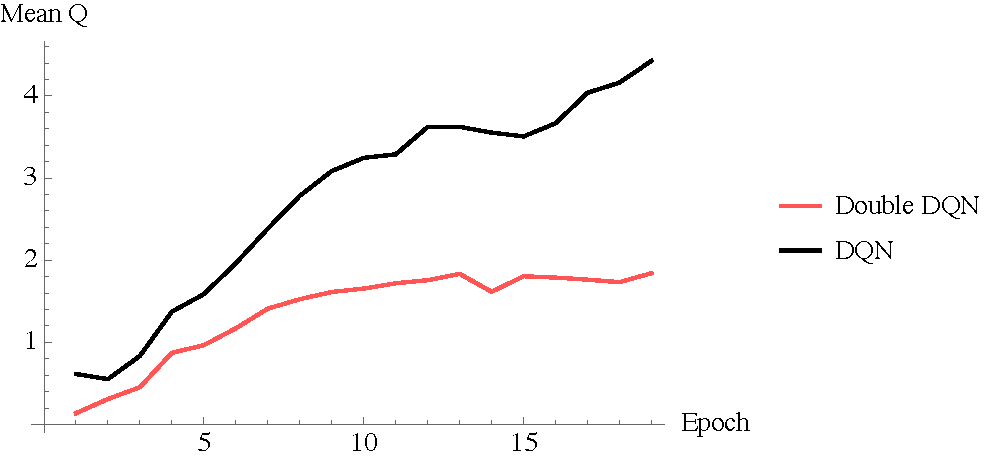
\includegraphics[width=120mm]{dqn_meanq.pdf}
  \end{figure}

  A member of the open source community, Alejandro Dubrovsky, was kind enough to run an evaluation on Space Invaders, both with and without Double Q learning:
  \begin{figure}[H]
    \centering
    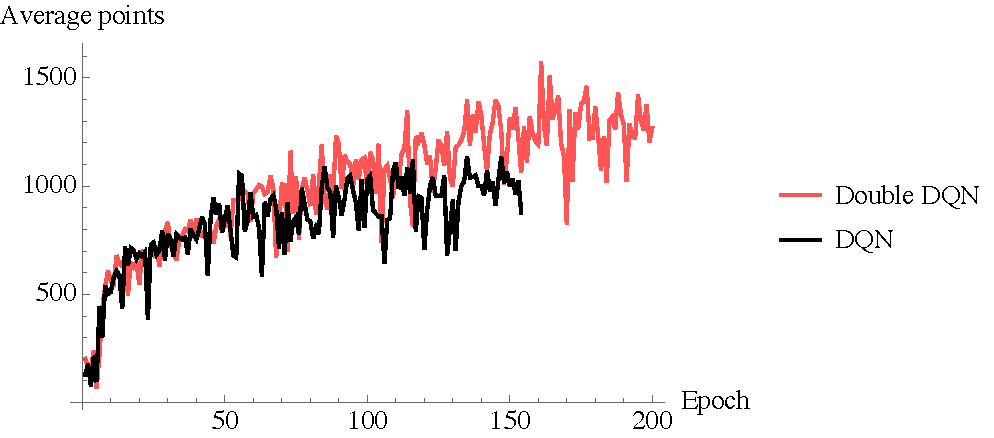
\includegraphics[width=120mm]{dqn_si_rewardper.pdf}
  \end{figure}
  \begin{figure}[H]
    \centering
    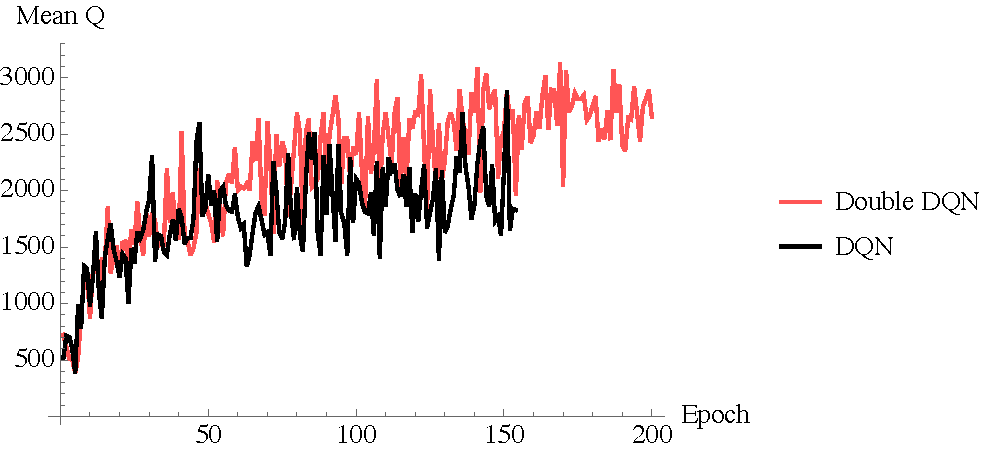
\includegraphics[width=120mm]{dqn_si_meanq.pdf}
  \end{figure}
  It seems clear that the implementation of Double Q learning performs better than previous implementations, at least in \texttt{deep\_q\_rl}. The average scores are higher, and the maximum scores are also higher. The maintainer of the codebase plans on merging in the changes this month.

\section{Design challenges}
The computational burden of Deep Q learning can be cost prohibitive on a small budget. The amount of computation also increases development turnaround time, since often only one set of changes can be tried in a day. \\

Put more design challenges here.

\section{Summary}
A summary goes here.


\begin{thebibliography}{1}
\bibitem{ale} Marc G. Bellemare, Yavar Naddaf, Joel Veness, and Michael Bowling. {\em The Arcade Learning Environment: An Evaluation Platform for General Agents}. In Journal of Artificial Intelligence Research 47, pp. 253-279, 2013.
\bibitem{dmnips} Mnih, V., Kavukcuoglu, K., Silver, D., Graves, A., Antonoglou, I., Wierstra, D., \& Riedmiller, M. (2013). Playing Atari with deep reinforcement learning. \textit{arXiv preprint arXiv:1312.5602}.
\bibitem{dmnature} Mnih, Volodymyr, et al. {\em Human-level control through deep reinforcement learning}. Nature 518.7540 (2015): 529-533.
\bibitem{sutton} R. S. Sutton and A. G. Barto, {\em Reinforcement Learning: An Introduction}. Cambridge, MA: MIT Press, 1998.
\bibitem{dmdoubl} van Hasselt, H., Guez, A., \& Silver, D. (2015). Deep Reinforcement Learning with Double Q-learning. \textit{arXiv preprint arXiv:1509.06461}.
\end{thebibliography}

%\section{Appendix}
%\begin{center}
  %\lstinputlisting{/Users/cwalker32/Documents/LaTeX/ece_517/proj2/et.m}
%\end{center}


\pagebreak

\end{document}
